% =========================================================
% % % =========================================================
% % % =========================================================
% % % =========================================================
% % \input{./diagrams/dia-Ch1/test-tikz.tex}
% =========================================================

%% TikZ is a very large program which can do lots of things. You will find commands to draw hierarchial trees, to draw lots of different types of shapes, to do some elementary programming, to align elements of a picture in a matrix frame, to decorate nodes, to compute the intersections of paths, etc.  The main message is “if it is not in these notes, it is most probably somewhere in the manual”


\begin{center}
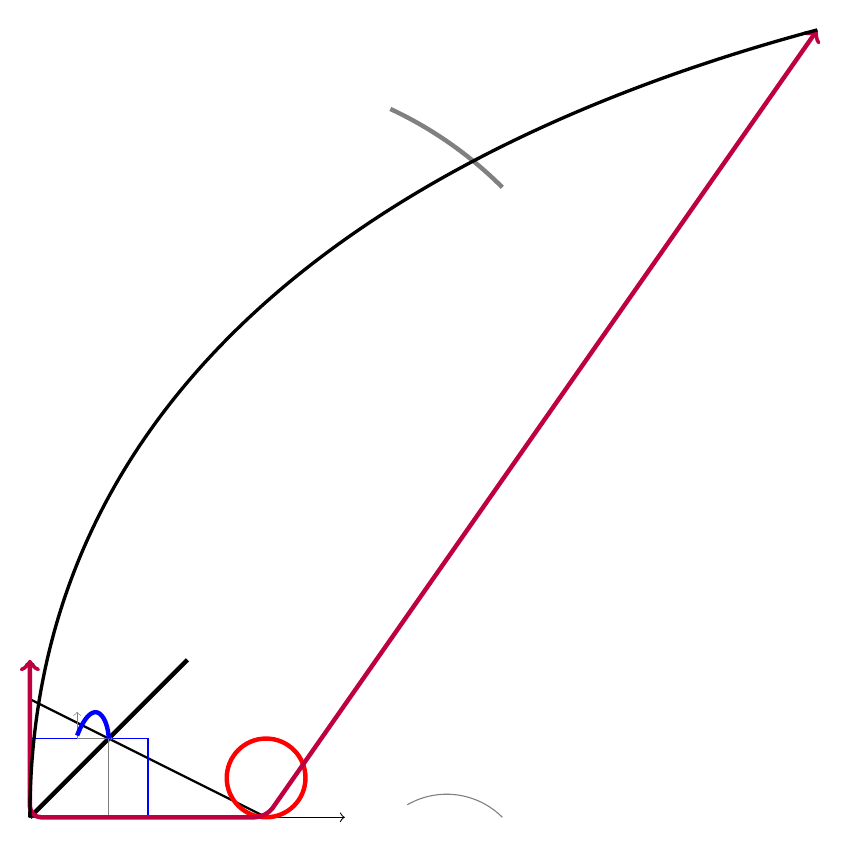
\begin{tikzpicture}

\draw [<->] (0,2) -- (0,0) -- (4,0);
\draw [thick] (0,1.5) -- (3,0);
\draw [ultra thick] (0,0) -- (2,2);
\draw [help lines] (1,0) -- (1,1) -- (0,1);

\draw [blue] (0,0) rectangle (1.5,1);
\draw [red, ultra thick] (3,0.5) circle [radius=0.5];;
\draw [gray] (6,0) arc [radius=1, start angle=45, end angle= 120];


\draw [<->, rounded corners, ultra thick, purple] (0,2) -- (0,0) -- (3,0) -- (10, 10);


\draw [gray, ultra thick] (6,8) arc [radius=5, start angle=45, end angle= 65];

\draw[very thick] (0,0) to [out=90,in=195] (10,10);

\draw [<->, help lines] (0.6,1.34) -- (0.6,1) -- (1.05,1);
\draw[blue, ultra thick] (0.6, 1.0385) -- (0.61, 1.06372) -- (0.62, 1.08756) -- (0.63, 1.11012) -- (0.64,1.13147) -- (0.65, 1.15166) -- (0.66, 1.17074) -- (0.67, 1.18874) -- (0.68,1.20568) -- (0.69, 1.22157) -- (0.7, 1.23643) -- (0.71, 1.25026) -- (0.72,1.26307) -- (0.73, 1.27486) -- (0.74, 1.28561) -- (0.75, 1.29534) -- (0.76, 1.30402) -- (0.77, 1.31165) -- (0.78, 1.31821) -- (0.79, 1.32369) -- (0.8, 1.32806) -- (0.81, 1.33131) -- (0.82, 1.3334) -- (0.83, 1.33431) -- (0.84, 1.334) -- (0.85, 1.33244) -- (0.86, 1.32956) -- (0.87, 1.32533) -- (0.88, 1.31966) -- (0.89, 1.3125) -- (0.9, 1.30373) -- (0.91, 1.29325) -- (0.92, 1.2809) -- (0.93, 1.26649) -- (0.94, 1.24976) -- (0.95, 1.23032) -- (0.96, 1.2076) -- (0.97, 1.18065) -- (0.98, 1.14763) -- (0.99, 1.1038) -- (0.991, 1.09836) -- (0.992, 1.09261) -- (0.993, 1.0865) -- (0.994, 1.07994) -- (0.995, 1.07282) -- (0.996, 1.06497) -- (0.997, 1.0561) -- (0.998, 1.04563) -- (0.999, 1.03209) -- (0.9991, 1.03042) -- (0.9992, 1.02866) -- (0.9993, 1.02679) -- (0.9994, 1.02478) -- (0.9995, 1.0226) -- (0.9996, 1.02019) -- (0.9997, 1.01747) -- (0.9998, 1.01424) -- (0.9999, 1.01005) -- (0.9999, 1.01005) -- (0.99991, 1.00953) -- (0.99992, 1.00898) -- (0.99993, 1.0084) -- (0.99994, 1.00778) -- (0.99995, 1.0071) -- (0.99996, 1.00634) -- (0.99997, 1.00549) -- (0.99998, 1.00448) -- (0.99999, 1.00317) -- (1,1);
\end{tikzpicture}
\end{center}


\begin{center}
\begin{tikzpicture}[domain=0:0.5,xscale=10,yscale=10]

\draw[<->] (0,2) node[left]{EUR}-- (0,0) -- (.7,0) node[below] {$q$};
\draw[red] plot (\x, {0.25+\x/2+\x*\x/2}) node[right] {$v_1(x)$};
\draw[green] plot (\x, {0.025+\x+\x*\x}) node[right] {$v_2(x)$};
\draw[thin, dashed] plot (\x, {0.275+1.5*\x+1.5*\x*\x}) ;
\draw[thick,domain=0:0.33666] plot (\x, {0.05+2*\x+2*\x*\x}) ;
\draw[thick,domain=0.33666:0.5]
plot (\x, {0.5+\x+\x*\x}) node[right] {$2\min[v_1,v_2]$};


\end{tikzpicture}
\end{center}

% =========================================================

%% TikZ is a very large program which can do lots of things. You will find commands to draw hierarchial trees, to draw lots of different types of shapes, to do some elementary programming, to align elements of a picture in a matrix frame, to decorate nodes, to compute the intersections of paths, etc.  The main message is “if it is not in these notes, it is most probably somewhere in the manual”


\begin{center}
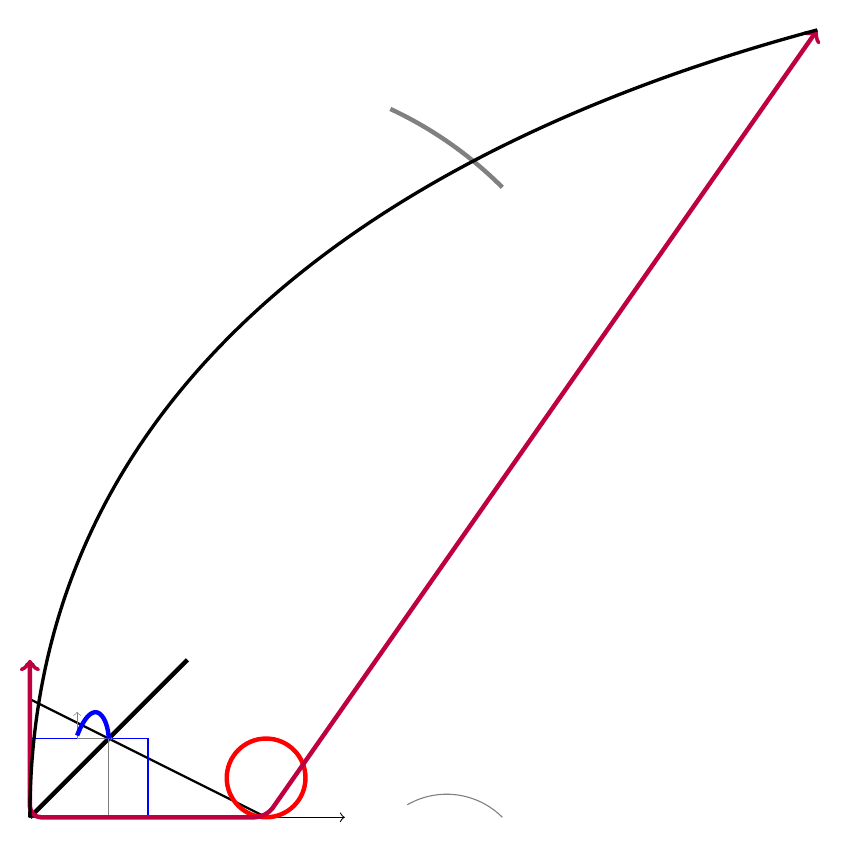
\begin{tikzpicture}

\draw [<->] (0,2) -- (0,0) -- (4,0);
\draw [thick] (0,1.5) -- (3,0);
\draw [ultra thick] (0,0) -- (2,2);
\draw [help lines] (1,0) -- (1,1) -- (0,1);

\draw [blue] (0,0) rectangle (1.5,1);
\draw [red, ultra thick] (3,0.5) circle [radius=0.5];;
\draw [gray] (6,0) arc [radius=1, start angle=45, end angle= 120];


\draw [<->, rounded corners, ultra thick, purple] (0,2) -- (0,0) -- (3,0) -- (10, 10);


\draw [gray, ultra thick] (6,8) arc [radius=5, start angle=45, end angle= 65];

\draw[very thick] (0,0) to [out=90,in=195] (10,10);

\draw [<->, help lines] (0.6,1.34) -- (0.6,1) -- (1.05,1);
\draw[blue, ultra thick] (0.6, 1.0385) -- (0.61, 1.06372) -- (0.62, 1.08756) -- (0.63, 1.11012) -- (0.64,1.13147) -- (0.65, 1.15166) -- (0.66, 1.17074) -- (0.67, 1.18874) -- (0.68,1.20568) -- (0.69, 1.22157) -- (0.7, 1.23643) -- (0.71, 1.25026) -- (0.72,1.26307) -- (0.73, 1.27486) -- (0.74, 1.28561) -- (0.75, 1.29534) -- (0.76, 1.30402) -- (0.77, 1.31165) -- (0.78, 1.31821) -- (0.79, 1.32369) -- (0.8, 1.32806) -- (0.81, 1.33131) -- (0.82, 1.3334) -- (0.83, 1.33431) -- (0.84, 1.334) -- (0.85, 1.33244) -- (0.86, 1.32956) -- (0.87, 1.32533) -- (0.88, 1.31966) -- (0.89, 1.3125) -- (0.9, 1.30373) -- (0.91, 1.29325) -- (0.92, 1.2809) -- (0.93, 1.26649) -- (0.94, 1.24976) -- (0.95, 1.23032) -- (0.96, 1.2076) -- (0.97, 1.18065) -- (0.98, 1.14763) -- (0.99, 1.1038) -- (0.991, 1.09836) -- (0.992, 1.09261) -- (0.993, 1.0865) -- (0.994, 1.07994) -- (0.995, 1.07282) -- (0.996, 1.06497) -- (0.997, 1.0561) -- (0.998, 1.04563) -- (0.999, 1.03209) -- (0.9991, 1.03042) -- (0.9992, 1.02866) -- (0.9993, 1.02679) -- (0.9994, 1.02478) -- (0.9995, 1.0226) -- (0.9996, 1.02019) -- (0.9997, 1.01747) -- (0.9998, 1.01424) -- (0.9999, 1.01005) -- (0.9999, 1.01005) -- (0.99991, 1.00953) -- (0.99992, 1.00898) -- (0.99993, 1.0084) -- (0.99994, 1.00778) -- (0.99995, 1.0071) -- (0.99996, 1.00634) -- (0.99997, 1.00549) -- (0.99998, 1.00448) -- (0.99999, 1.00317) -- (1,1);
\end{tikzpicture}
\end{center}


\begin{center}
\begin{tikzpicture}[domain=0:0.5,xscale=10,yscale=10]

\draw[<->] (0,2) node[left]{EUR}-- (0,0) -- (.7,0) node[below] {$q$};
\draw[red] plot (\x, {0.25+\x/2+\x*\x/2}) node[right] {$v_1(x)$};
\draw[green] plot (\x, {0.025+\x+\x*\x}) node[right] {$v_2(x)$};
\draw[thin, dashed] plot (\x, {0.275+1.5*\x+1.5*\x*\x}) ;
\draw[thick,domain=0:0.33666] plot (\x, {0.05+2*\x+2*\x*\x}) ;
\draw[thick,domain=0.33666:0.5]
plot (\x, {0.5+\x+\x*\x}) node[right] {$2\min[v_1,v_2]$};


\end{tikzpicture}
\end{center}

% =========================================================

%% TikZ is a very large program which can do lots of things. You will find commands to draw hierarchial trees, to draw lots of different types of shapes, to do some elementary programming, to align elements of a picture in a matrix frame, to decorate nodes, to compute the intersections of paths, etc.  The main message is “if it is not in these notes, it is most probably somewhere in the manual”


\begin{center}
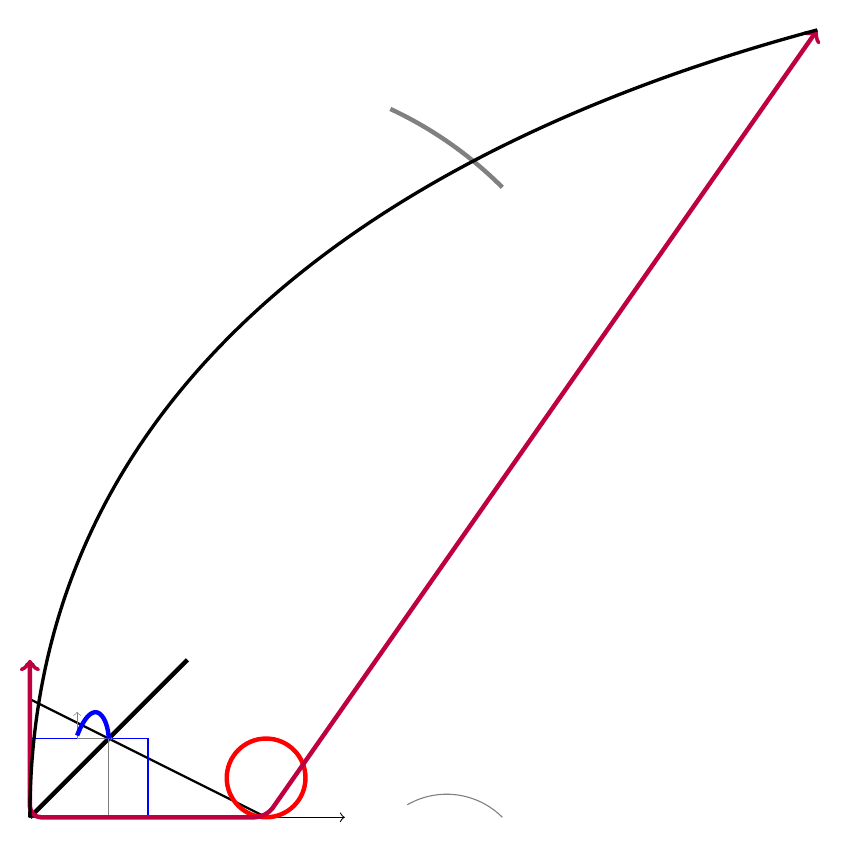
\begin{tikzpicture}

\draw [<->] (0,2) -- (0,0) -- (4,0);
\draw [thick] (0,1.5) -- (3,0);
\draw [ultra thick] (0,0) -- (2,2);
\draw [help lines] (1,0) -- (1,1) -- (0,1);

\draw [blue] (0,0) rectangle (1.5,1);
\draw [red, ultra thick] (3,0.5) circle [radius=0.5];;
\draw [gray] (6,0) arc [radius=1, start angle=45, end angle= 120];


\draw [<->, rounded corners, ultra thick, purple] (0,2) -- (0,0) -- (3,0) -- (10, 10);


\draw [gray, ultra thick] (6,8) arc [radius=5, start angle=45, end angle= 65];

\draw[very thick] (0,0) to [out=90,in=195] (10,10);

\draw [<->, help lines] (0.6,1.34) -- (0.6,1) -- (1.05,1);
\draw[blue, ultra thick] (0.6, 1.0385) -- (0.61, 1.06372) -- (0.62, 1.08756) -- (0.63, 1.11012) -- (0.64,1.13147) -- (0.65, 1.15166) -- (0.66, 1.17074) -- (0.67, 1.18874) -- (0.68,1.20568) -- (0.69, 1.22157) -- (0.7, 1.23643) -- (0.71, 1.25026) -- (0.72,1.26307) -- (0.73, 1.27486) -- (0.74, 1.28561) -- (0.75, 1.29534) -- (0.76, 1.30402) -- (0.77, 1.31165) -- (0.78, 1.31821) -- (0.79, 1.32369) -- (0.8, 1.32806) -- (0.81, 1.33131) -- (0.82, 1.3334) -- (0.83, 1.33431) -- (0.84, 1.334) -- (0.85, 1.33244) -- (0.86, 1.32956) -- (0.87, 1.32533) -- (0.88, 1.31966) -- (0.89, 1.3125) -- (0.9, 1.30373) -- (0.91, 1.29325) -- (0.92, 1.2809) -- (0.93, 1.26649) -- (0.94, 1.24976) -- (0.95, 1.23032) -- (0.96, 1.2076) -- (0.97, 1.18065) -- (0.98, 1.14763) -- (0.99, 1.1038) -- (0.991, 1.09836) -- (0.992, 1.09261) -- (0.993, 1.0865) -- (0.994, 1.07994) -- (0.995, 1.07282) -- (0.996, 1.06497) -- (0.997, 1.0561) -- (0.998, 1.04563) -- (0.999, 1.03209) -- (0.9991, 1.03042) -- (0.9992, 1.02866) -- (0.9993, 1.02679) -- (0.9994, 1.02478) -- (0.9995, 1.0226) -- (0.9996, 1.02019) -- (0.9997, 1.01747) -- (0.9998, 1.01424) -- (0.9999, 1.01005) -- (0.9999, 1.01005) -- (0.99991, 1.00953) -- (0.99992, 1.00898) -- (0.99993, 1.0084) -- (0.99994, 1.00778) -- (0.99995, 1.0071) -- (0.99996, 1.00634) -- (0.99997, 1.00549) -- (0.99998, 1.00448) -- (0.99999, 1.00317) -- (1,1);
\end{tikzpicture}
\end{center}


\begin{center}
\begin{tikzpicture}[domain=0:0.5,xscale=10,yscale=10]

\draw[<->] (0,2) node[left]{EUR}-- (0,0) -- (.7,0) node[below] {$q$};
\draw[red] plot (\x, {0.25+\x/2+\x*\x/2}) node[right] {$v_1(x)$};
\draw[green] plot (\x, {0.025+\x+\x*\x}) node[right] {$v_2(x)$};
\draw[thin, dashed] plot (\x, {0.275+1.5*\x+1.5*\x*\x}) ;
\draw[thick,domain=0:0.33666] plot (\x, {0.05+2*\x+2*\x*\x}) ;
\draw[thick,domain=0.33666:0.5]
plot (\x, {0.5+\x+\x*\x}) node[right] {$2\min[v_1,v_2]$};


\end{tikzpicture}
\end{center}

% =========================================================

%% TikZ is a very large program which can do lots of things. You will find commands to draw hierarchial trees, to draw lots of different types of shapes, to do some elementary programming, to align elements of a picture in a matrix frame, to decorate nodes, to compute the intersections of paths, etc.  The main message is “if it is not in these notes, it is most probably somewhere in the manual”


\begin{center}
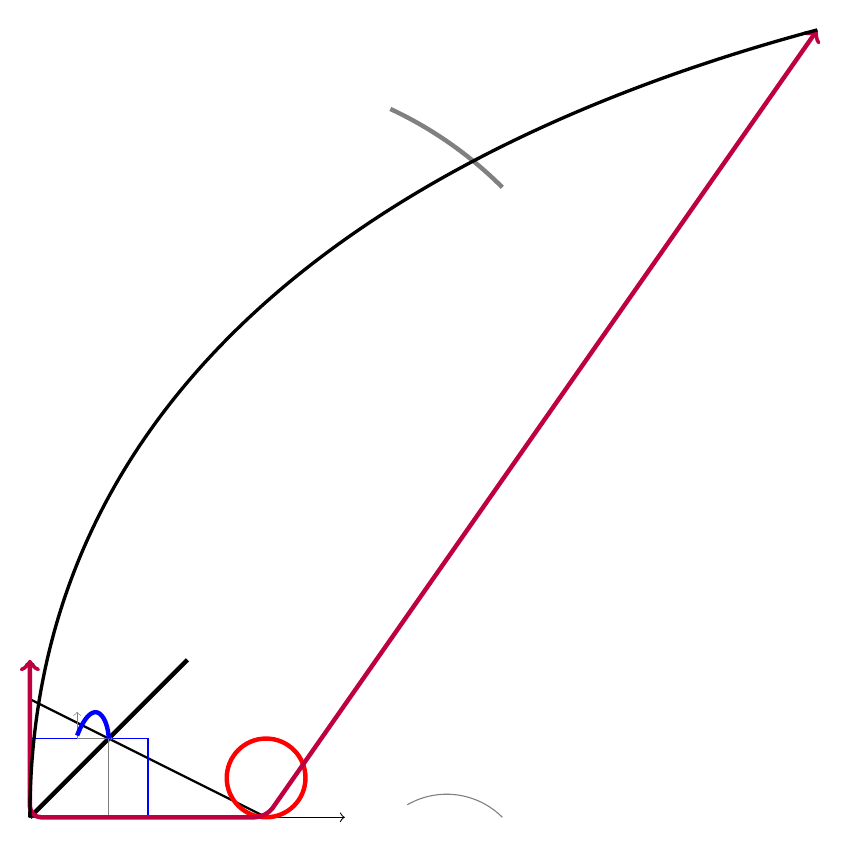
\begin{tikzpicture}

\draw [<->] (0,2) -- (0,0) -- (4,0);
\draw [thick] (0,1.5) -- (3,0);
\draw [ultra thick] (0,0) -- (2,2);
\draw [help lines] (1,0) -- (1,1) -- (0,1);

\draw [blue] (0,0) rectangle (1.5,1);
\draw [red, ultra thick] (3,0.5) circle [radius=0.5];;
\draw [gray] (6,0) arc [radius=1, start angle=45, end angle= 120];


\draw [<->, rounded corners, ultra thick, purple] (0,2) -- (0,0) -- (3,0) -- (10, 10);


\draw [gray, ultra thick] (6,8) arc [radius=5, start angle=45, end angle= 65];

\draw[very thick] (0,0) to [out=90,in=195] (10,10);

\draw [<->, help lines] (0.6,1.34) -- (0.6,1) -- (1.05,1);
\draw[blue, ultra thick] (0.6, 1.0385) -- (0.61, 1.06372) -- (0.62, 1.08756) -- (0.63, 1.11012) -- (0.64,1.13147) -- (0.65, 1.15166) -- (0.66, 1.17074) -- (0.67, 1.18874) -- (0.68,1.20568) -- (0.69, 1.22157) -- (0.7, 1.23643) -- (0.71, 1.25026) -- (0.72,1.26307) -- (0.73, 1.27486) -- (0.74, 1.28561) -- (0.75, 1.29534) -- (0.76, 1.30402) -- (0.77, 1.31165) -- (0.78, 1.31821) -- (0.79, 1.32369) -- (0.8, 1.32806) -- (0.81, 1.33131) -- (0.82, 1.3334) -- (0.83, 1.33431) -- (0.84, 1.334) -- (0.85, 1.33244) -- (0.86, 1.32956) -- (0.87, 1.32533) -- (0.88, 1.31966) -- (0.89, 1.3125) -- (0.9, 1.30373) -- (0.91, 1.29325) -- (0.92, 1.2809) -- (0.93, 1.26649) -- (0.94, 1.24976) -- (0.95, 1.23032) -- (0.96, 1.2076) -- (0.97, 1.18065) -- (0.98, 1.14763) -- (0.99, 1.1038) -- (0.991, 1.09836) -- (0.992, 1.09261) -- (0.993, 1.0865) -- (0.994, 1.07994) -- (0.995, 1.07282) -- (0.996, 1.06497) -- (0.997, 1.0561) -- (0.998, 1.04563) -- (0.999, 1.03209) -- (0.9991, 1.03042) -- (0.9992, 1.02866) -- (0.9993, 1.02679) -- (0.9994, 1.02478) -- (0.9995, 1.0226) -- (0.9996, 1.02019) -- (0.9997, 1.01747) -- (0.9998, 1.01424) -- (0.9999, 1.01005) -- (0.9999, 1.01005) -- (0.99991, 1.00953) -- (0.99992, 1.00898) -- (0.99993, 1.0084) -- (0.99994, 1.00778) -- (0.99995, 1.0071) -- (0.99996, 1.00634) -- (0.99997, 1.00549) -- (0.99998, 1.00448) -- (0.99999, 1.00317) -- (1,1);
\end{tikzpicture}
\end{center}


\begin{center}
\begin{tikzpicture}[domain=0:0.5,xscale=10,yscale=10]

\draw[<->] (0,2) node[left]{EUR}-- (0,0) -- (.7,0) node[below] {$q$};
\draw[red] plot (\x, {0.25+\x/2+\x*\x/2}) node[right] {$v_1(x)$};
\draw[green] plot (\x, {0.025+\x+\x*\x}) node[right] {$v_2(x)$};
\draw[thin, dashed] plot (\x, {0.275+1.5*\x+1.5*\x*\x}) ;
\draw[thick,domain=0:0.33666] plot (\x, {0.05+2*\x+2*\x*\x}) ;
\draw[thick,domain=0.33666:0.5]
plot (\x, {0.5+\x+\x*\x}) node[right] {$2\min[v_1,v_2]$};


\end{tikzpicture}
\end{center}
